\section{Design and Implementation}
\subsection{Power Stage Calculation and Component Selection}
Design of a 120W flyback Converter Operating in Continuous Conduction Mode (CCM) with
the following specifications:
\newpage
\begin{table}[h!]
    \centering
    \begin{tabular}{l l l}
        \toprule
        \textbf{Parameter} & \textbf{Symbol} & \textbf{Value} \\
        \midrule
        Input Voltage & $ V_{in} $ & 310 V \\
        Output Voltage & $ V_{out} $ & 24 V \\
        Output Power & $ P_{out} $ & 100 W \\
        Switching Frequency & $ f_{sw} $ & 100 kHz \\
        Diode Voltage & $ V_d $ & 1 V \\
        Ripple Current Rate & - & 30\% \\
        Ripple Voltage Rate & - & 1\% \\
        Duty Cycle & $ D $ & 30\%\\
        efficiency & $ \eta $ & 90\%\\
        \bottomrule
    \end{tabular}
    \caption{Input Parameters}
\end{table}
\subsection{Power Stage Calculations}
\subsubsection*{1. Transformer Turn Ratio}
\[
\frac{N_p}{N_s} = \frac{V_{in} \cdot D}{(V_{out} + V_f)(1 - D)} 
= \frac{310 \cdot 0.3}{(24 + 1) \cdot 0.7} \approx \boxed{5.314:1}
\]
\subsubsection*{2. Output Current}
\[
I_{out} = \frac{P_{out}}{V_{out}} = \frac{100}{24} \approx \boxed{4.167\,\text{A}}
\]
\subsection*{3. Load Resistance}
\[
R_{\text{load}} = \frac{V_{out}}{I_{out}} = \frac{24}{4.167} \approx \boxed{5.76\,\Omega}
\]
\subsection*{$\bullet$ Transformer Primary Side Calculation}
\subsubsection*{4. Primary Average Current}
\[
I_{\text{primary\_avg}} = \frac{P_{in}}{V_{in} \cdot D} 
= \frac{111.11}{310 \cdot 0.3} \approx \boxed{1.195\,\text{A}}
\]
\subsubsection*{5. Primary Ripple Current}
\[
\Delta I_{L1} = 0.3 \cdot I_{\text{primary\_avg}} = 0.3 \cdot 1.195 \approx \boxed{0.358\,\text{A (p-p)}}
\]
\subsubsection*{6. Primary Maximum Current}
\[
I_{\text{primary\_max}} = I_{\text{primary\_avg}} + \frac{\Delta I_{L1}}{2} 
\approx 1.195 + 0.179 \approx \boxed{1.374\,\text{A}} 
\]
\subsubsection*{7. Primary Minimum Current}
\[
I_{\text{primary\_min}} = I_{\text{primary\_avg}} - \frac{\Delta I_{L1}}{2} 
\approx 1.195 - 0.179 \approx \boxed{1.016\,\text{A}} \\
\]
\subsubsection*{8. Primary rms Current}
\[
I_{\text{primary\_rms}} = \sqrt{\frac{1}{3} \left( I_{\text{primary\_peak}}^2 + I_{\text{primary\_peak}}I_{\text{primary\_min}} + I_{\text{primary\_min}}^2 \right)} 
\approx \boxed{1.21\,\text{A}}
\]
\subsubsection*{9. Magnetizing Inductance or Primary Inductance}
\[
L_p = \frac{V_{in} \cdot D}{\Delta I_{L1} \cdot f_{sw}} 
= \frac{310 \cdot 0.3}{0.358 \cdot 100 \cdot 10^3} \approx \boxed{2.595\,\text{mH}}
\]
\subsection*{$\bullet$ Transformer Secondary Side Calculation}
\subsubsection*{10. Secondary Average Current}
\[
I_{\text{secondary\_avg}} = I_{out} = \boxed{4.167\,\text{A}}
\]
\subsubsection*{11. Secondary Ripple Current}
\[
\Delta I_{\text{secondary}} = \Delta I_{L1} \cdot I_{\text{secondary\_avg}} =0.358 \cdot 5.314 = \boxed{1.9332}
\]
\subsubsection*{12. Secondary Maximum Current }
\[
I_{\text{secondary\_max}} = I_{\text{primary\_max}} \cdot \frac{N_p}{N_s} 
\approx 1.374 \cdot 5.314 \approx \boxed{7.30\,\text{A}} \\
\]
\subsubsection*{13. Secondary Minimum Current}
\[
I_{\text{secondary\_min}} = I_{\text{secondary\_peak}} - \Delta I_{\text{secondary}} \\
= 7.30 - (0.358 \cdot 5.314) \approx \boxed{5.40\,\text{A}} \\
\]
\subsubsection*{14. Secondary rms Current}
\[
I_{\text{secondary\_rms}} = \sqrt{\frac{1}{3} \left( I_{\text{secondary\_max}}^2 + I_{\text{secondary\_max}}I_{\text{secondary\_min}} + I_{\text{secondary\_min}}^2 \right) \cdot (1 - D)} 
\approx \boxed{5.33\,\text{A}}
\]
\subsubsection*{15. Secondary Inductance}
\[
L_s = L_p \cdot \left( \frac{N_s}{N_p} \right)^2 
= 2.595 \cdot \left( \frac{1}{5.314} \right)^2 \approx \boxed{91.7\,\mu\text{H}}
\]
\subsection*{$\bullet$ Output Capacitor}
\subsubsection*{16. Ripple Output Voltage}
\[
\Delta V_{ripple} = 0.1 \cdot V_{out} = 0.1 \cdot 24 = \boxed{0.24V}
\]
\subsubsection*{17. Output Capacitor}
\[
C = \frac{I_{out} \cdot D}{f_{sw} \cdot \Delta V_{\text{ripple}}} 
= \frac{4.167 \cdot 0.3}{100 \cdot 10^3 \cdot 0.24} \approx \boxed{52.09\,\mu\text{F}}
\]
\subsection*{$\bullet$ Component Selection}
\subsubsection*{18. MOSFET}
\begin{center}
    \begin{minipage}{0.4\textwidth}
        \centering
        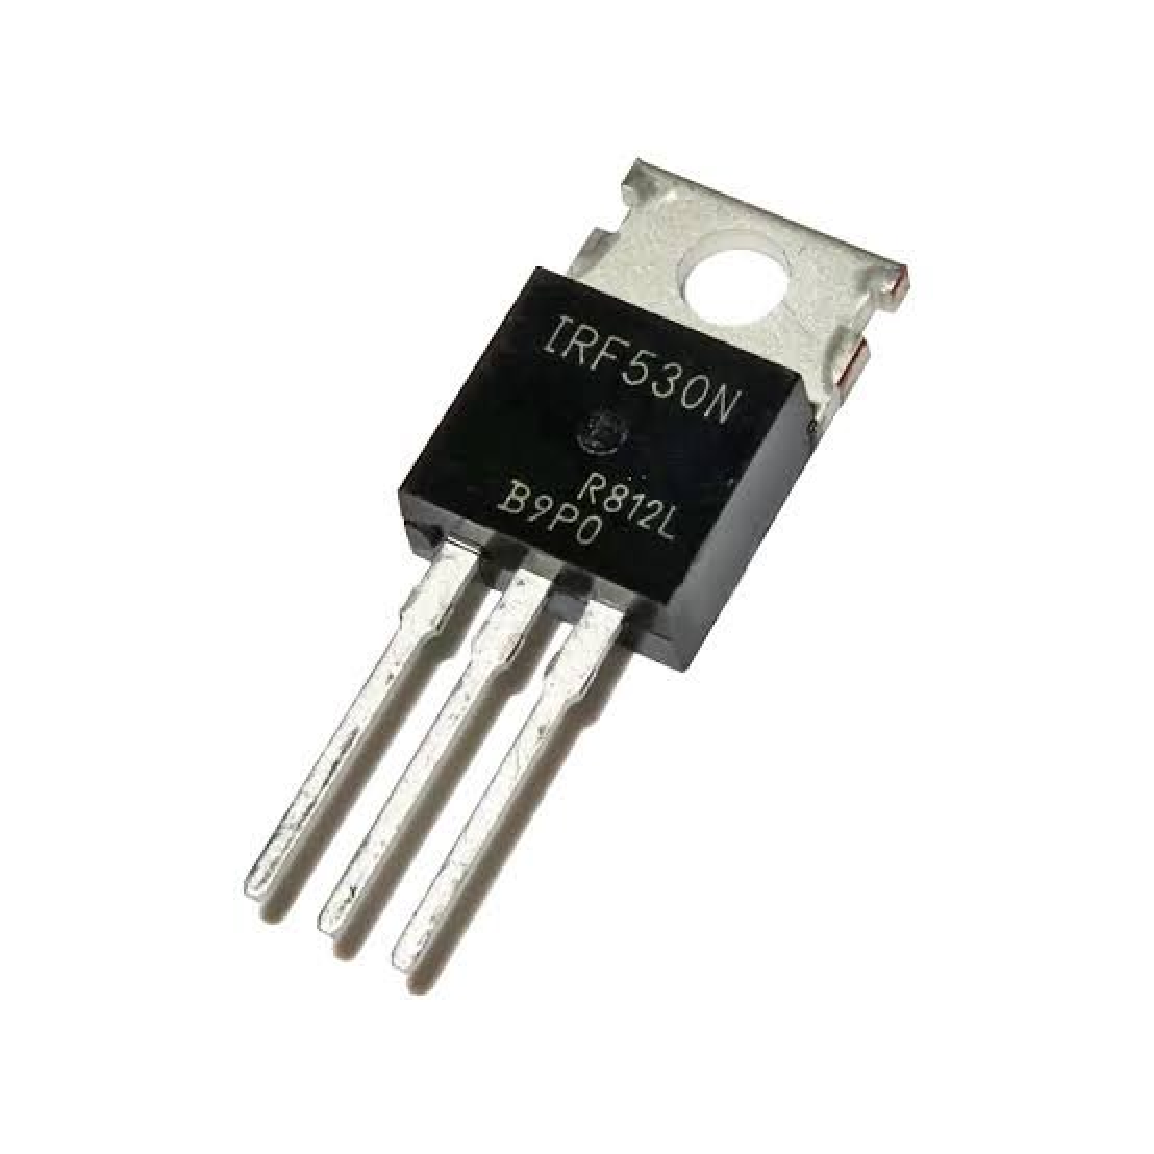
\includegraphics[width=0.8\linewidth]{Pictures/pics/mosfet.pdf} % Replace with your image file
        %\captionof{figure}{This is a figure.} % Add a caption
    \end{minipage}
    \hfill % Adds space between the minipages
    \begin{minipage}{0.55\textwidth}
    \centering
    \captionof{table}{IRF540N MOSFET}
    \label{tab:IRF530}
    \begin{tabular}{lcc}
    \toprule
    \footnotesize
    \textbf{Parameter} & \textbf{Value} & \textbf{Test Conditions} \\
    \midrule
     $V_{DS}$ & \SI{100}{\volt} & Absolute Maximum Rating \\
     $I_D$ & \SI{14}{\ampere} & $T_C = \SI{25}{\celsius}$ \\
     & \SI{10}{\ampere} & $T_C = \SI{100}{\celsius}$ \\
     $R_{DS(on)}$ & \SI{0.16}{\ohm} & $V_{GS} = \SI{10}{\volt}, I_D = \SI{8.4}{\ampere}$ \\
    \bottomrule
    \end{tabular}
    \end{minipage}
\end{center}
\subsubsection*{19. Diode Selection}
\begin{center}
    \begin{minipage}{0.4\textwidth}
        \centering
        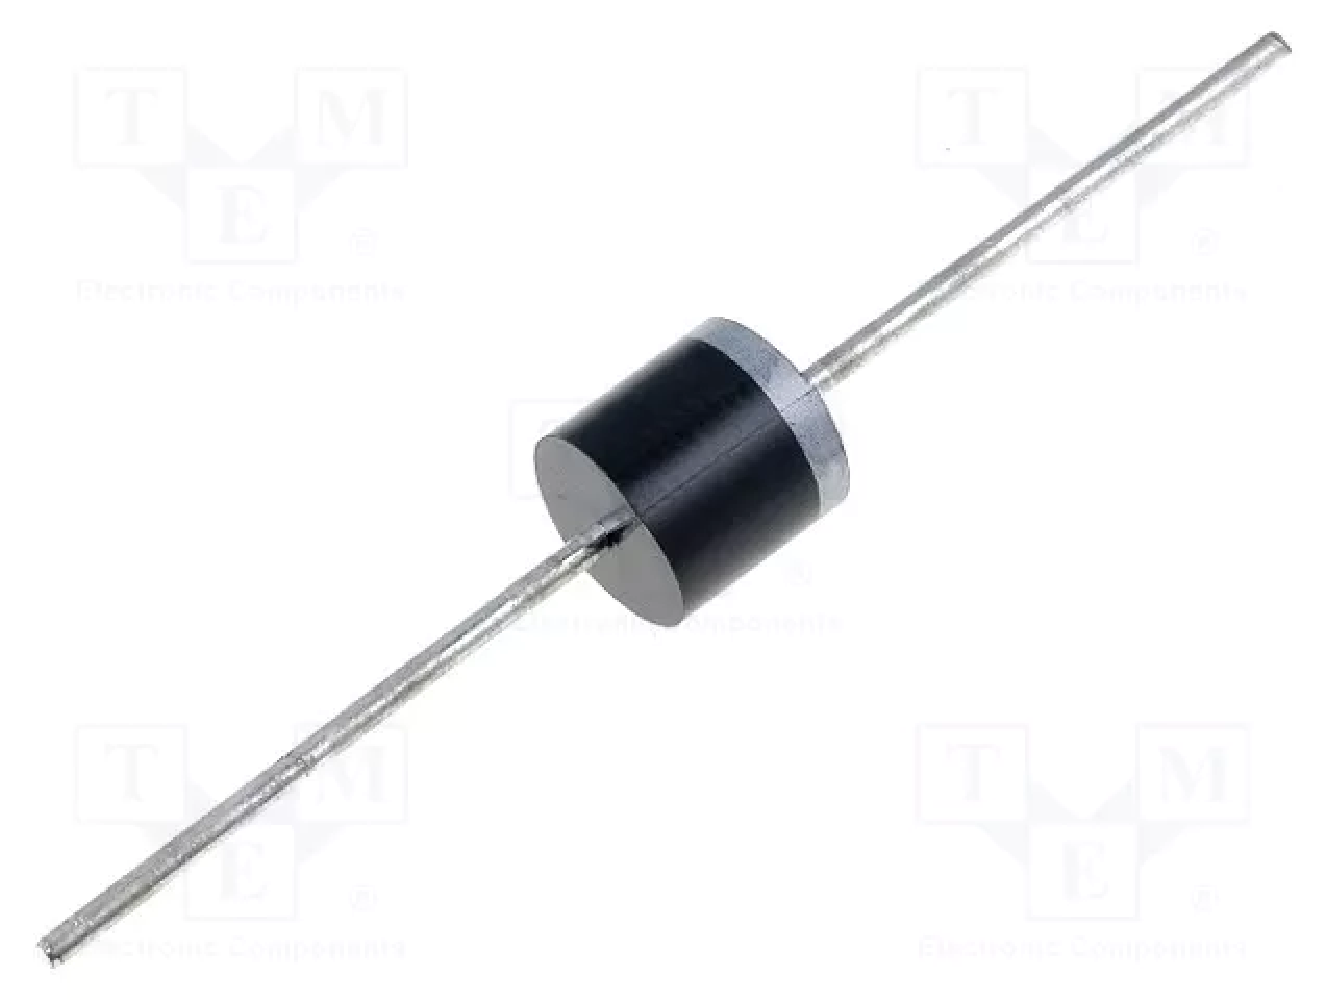
\includegraphics[width=0.7\linewidth]{Pictures/pics/diode.pdf} % Replace with your image file
        %\captionof{figure}{This is a figure.} % Add a caption
    \end{minipage}
    \hfill % Adds space between the minipages
    \begin{minipage}{0.55\textwidth}
    \centering
    \captionof{table}{15SQ045 Schottky Diode}
        \label{tab:SR510}
        \begin{tabular}{lcc}
        \toprule
        \textbf{Parameter} & \textbf{Value} & \textbf{Test Conditions} \\
        \midrule
        $V_{RRM}$ & \SI{100}{\volt} & Maximum repetitive rating \\
        $I_F$ & \SI{5}{\ampere} & Continuous, $T_A = \SI{25}{\celsius}$ \\
        \bottomrule
        \end{tabular}
    \end{minipage}
\end{center}
\subsection*{$\bullet$ Transformer Design}
\begin{table}[h!]
 \caption{Input Parameters for Flyback Transformer Design}
    \label{tab:input_parameters}
    \centering
    \begin{tabular}{l l l}
    \toprule
    \textbf{Parameter} & \textbf{Value} & \textbf{Unit} \\
    \midrule
    Inductance ($L$) & $\SI{2.955e-3}{}$ & \si{\henry} \\
    Primary Peak Current ($I_{p,\text{pk}}$) & $\SI{1.374}{}$ & \si{\ampere} \\
    Output Power ($P_o$) & $\SI{100}{}$ & \si{\watt} \\
    Ferrite Core Flux Density ($B_m$) & $\SI{0.25}{}$ & \si{\tesla} \\
    Regulation ($\alpha$) & $1$ & - \\
    Diode Drop Voltage ($V_d$) & $\SI{1}{}$ & \si{\volt} \\
    Duty Cycle ($D$) & $0.3$ & - \\
    Dwell Time Ratio ($D_w$) & $0.1$ & - \\
    Window Utilization ($K_u$) & $0.4$ & - \\
    Switching Frequency ($F$) & $\SI{100e3}{}$ & \si{\hertz} \\
    \bottomrule
    \end{tabular}
\end{table}
\subsubsection*{Energy-Handling Capability ($E$)}
\[
E = \frac{L \cdot I_{p,\text{pk}}^2}{2} = \frac{(2.955 \times 10^{-3}) \cdot (1.374)^2}{2} = \frac{(2.955 \times 10^{-3}) \cdot 1.887}{2} \approx \SI{0.00278}{\watt\second}
\]
\subsubsection*{Electrical Condition ($K_e$)}
\[
K_e = 0.145 \cdot P_o \cdot B_m^2 \cdot 10^{-4} = 0.145 \cdot 100 \cdot (0.25)^2 \cdot 10^{-4} = 9.0625 \times 10^{-5}
\]
\subsubsection*{Core Geometry ($K_g$)}
\[
K_g = \frac{E^2}{K_e \cdot \alpha} = \frac{(0.00278)^2}{9.0625 \times 10^{-5}} = \frac{7.7284 \times 10^{-6}}{9.0625 \times 10^{-5}} \approx 0.0853
\]
\begin{figure}[h!]
    \centering
    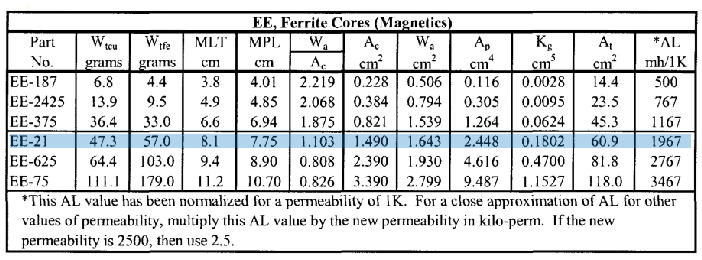
\includegraphics[width=1\linewidth]{Pictures/pics/EE21_selected.pdf}
    \caption{\textcolor{blue}{\textit{\footnotesize PQ Core Parameter Table List}}}
\end{figure} 
\begin{figure}[h!]
    \centering
    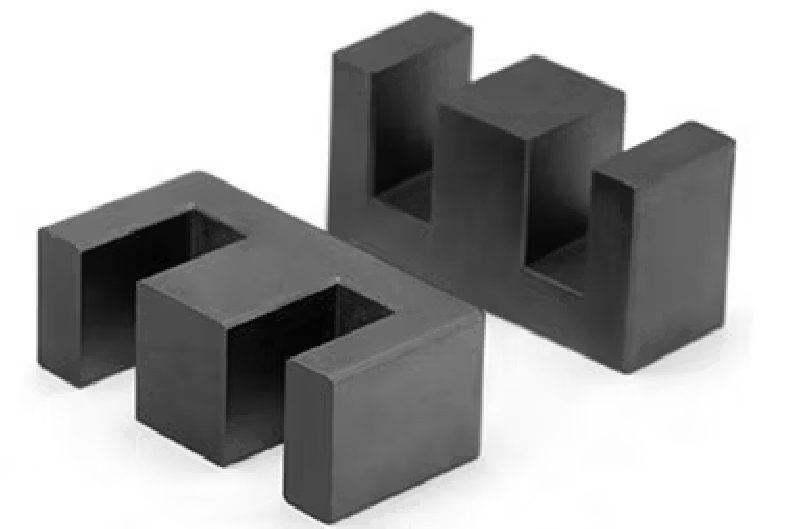
\includegraphics[width=0.5\linewidth]{Pictures/pics/eecore.pdf}
    \caption{\textcolor{blue}{\textit{\footnotesize EE21 Core}}}
\end{figure} 
\begin{table}[h!]
\centering
\begin{tabular}{l l l}
\toprule
\textbf{Parameter} & \textbf{Value} & \textbf{Unit} \\
\midrule
Magnetic Path Length ($MPL$) & $\SI{7.75}{}$ & \si{\centi\meter} \\
Core Weight ($W_{\text{core}}$) & $\SI{57}{}$ & \si{\gram} \\
Copper Weight ($W_{\text{copper}}$) & $\SI{47.3}{}$ & \si{\gram} \\
Mean Length Turn ($MLT$) & $\SI{8.1}{}$ & \si{\centi\meter} \\
Cross-Sectional Area ($A_c$) & $\SI{1.490}{}$ & \si{\centi\meter\squared} \\
Window Area ($W_a$) & $\SI{1.643}{}$ & \si{\centi\meter\squared} \\
Core Product ($A_p$) & $\SI{2.448}{}$ & \si{\centi\meter\tothe{4}} \\
Core Geometry ($Kg_s$) & $\SI{0.1802}{}$ & \si{\centi\meter\tothe{5}} \\
\bottomrule
\end{tabular}
\caption{Selected Core Parameters for Transformer Design}
\label{tab:core_parameters}
\end{table}
\subsubsection*{Current Density ($J$)}
\[
J = \frac{2 \cdot E \cdot 10^4}{B_m \cdot A_p \cdot K_u} = \frac{2 \cdot 0.00278 \cdot 10^4}{0.25 \cdot 2.448 \cdot 0.4} \approx \SI{227.1}{\ampere\per\centi\meter\squared}
\]
\subsubsection*{Primary Wire Area ($A_{pw}$)}
\[
A_{pw} = \frac{I_{p,\text{rms}}}{J} = \frac{1.21}{227.1} \approx \SI{0.00428}{\centi\meter\squared}
\]
\subsubsection*{Number of Primary Turns ($N_p$)}
\[
N_p = \frac{K_u \cdot W_a / 2}{3 \cdot A_{ws}} = \frac{0.4 \cdot (1.643 / 2)}{3 \cdot 0.01} \approx 11
\]
\subsubsection*{Secondary Wire Area ($A_{sw}$)}
\[
A_{sw} = \frac{I_{s,\text{rms}}}{J} = \frac{5.33}{227.1} \approx \SI{0.0227}{\centi\meter\squared}
\]
\subsubsection*{Secondary Turns ($N_s$)}
\[
N_s = \frac{N_p \cdot (V_o + V_d) \cdot (1 - D - D_w)}{V_i \cdot D} = \frac{11 \cdot (24 + 1) \cdot (1 - 0.3 - 0.1)}{310 \cdot 0.3} \approx 2
\]
\subsubsection*{Gap Length ($L_g$)}
\[
L_g = \left| \frac{0.4 \cdot \pi \cdot N_p^2 \cdot A_c \cdot 10^{-8}}{L} - \frac{MPL}{\mu_0} \right| = \left| \frac{0.4 \cdot \pi \cdot 11^2 \cdot 1.490 \cdot 10^{-8}}{2.955 \times 10^{-3}} - \frac{7.75}{2500} \right| \approx \SI{0.00453}{\centi\meter}
\]
\subsection{Flyback Convert Simulation}
\begin{figure}[h!]
    \centering
    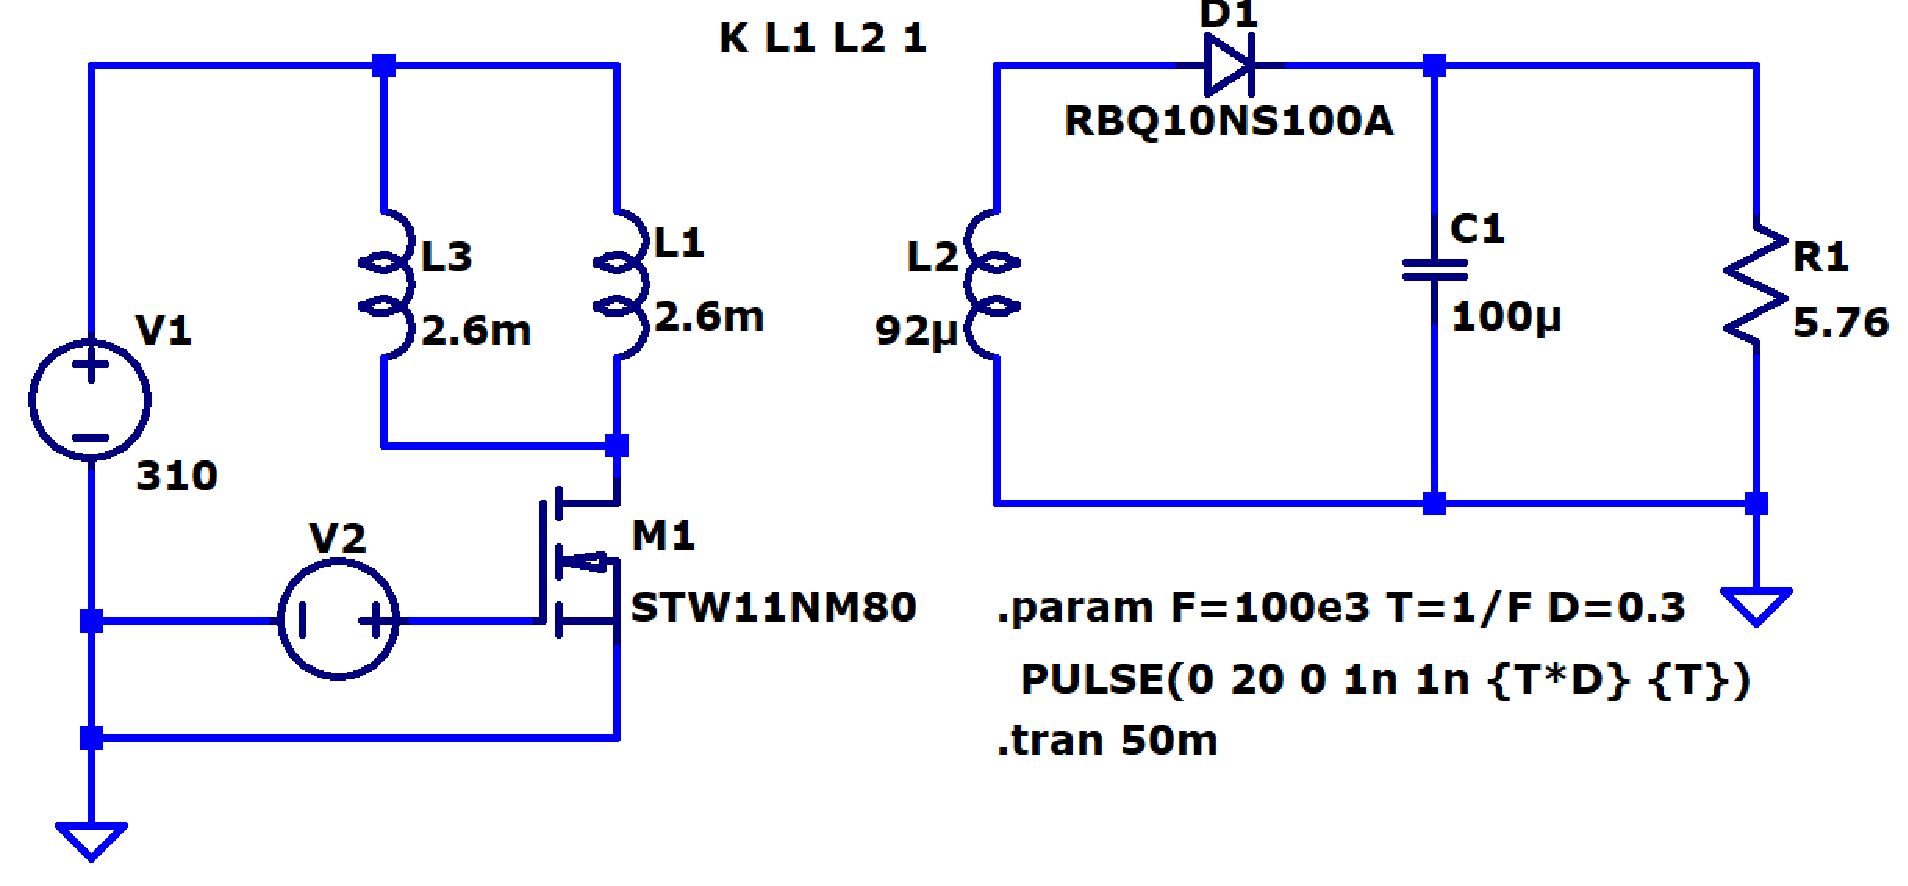
\includegraphics[width=0.8\linewidth]{Pictures/pics/LT_schem.pdf}
    \caption{\textcolor{blue}{\textit{\footnotesize Flyback Converter Schematic on LTspice}}}
\end{figure}
\begin{figure}[h!]
    \centering
    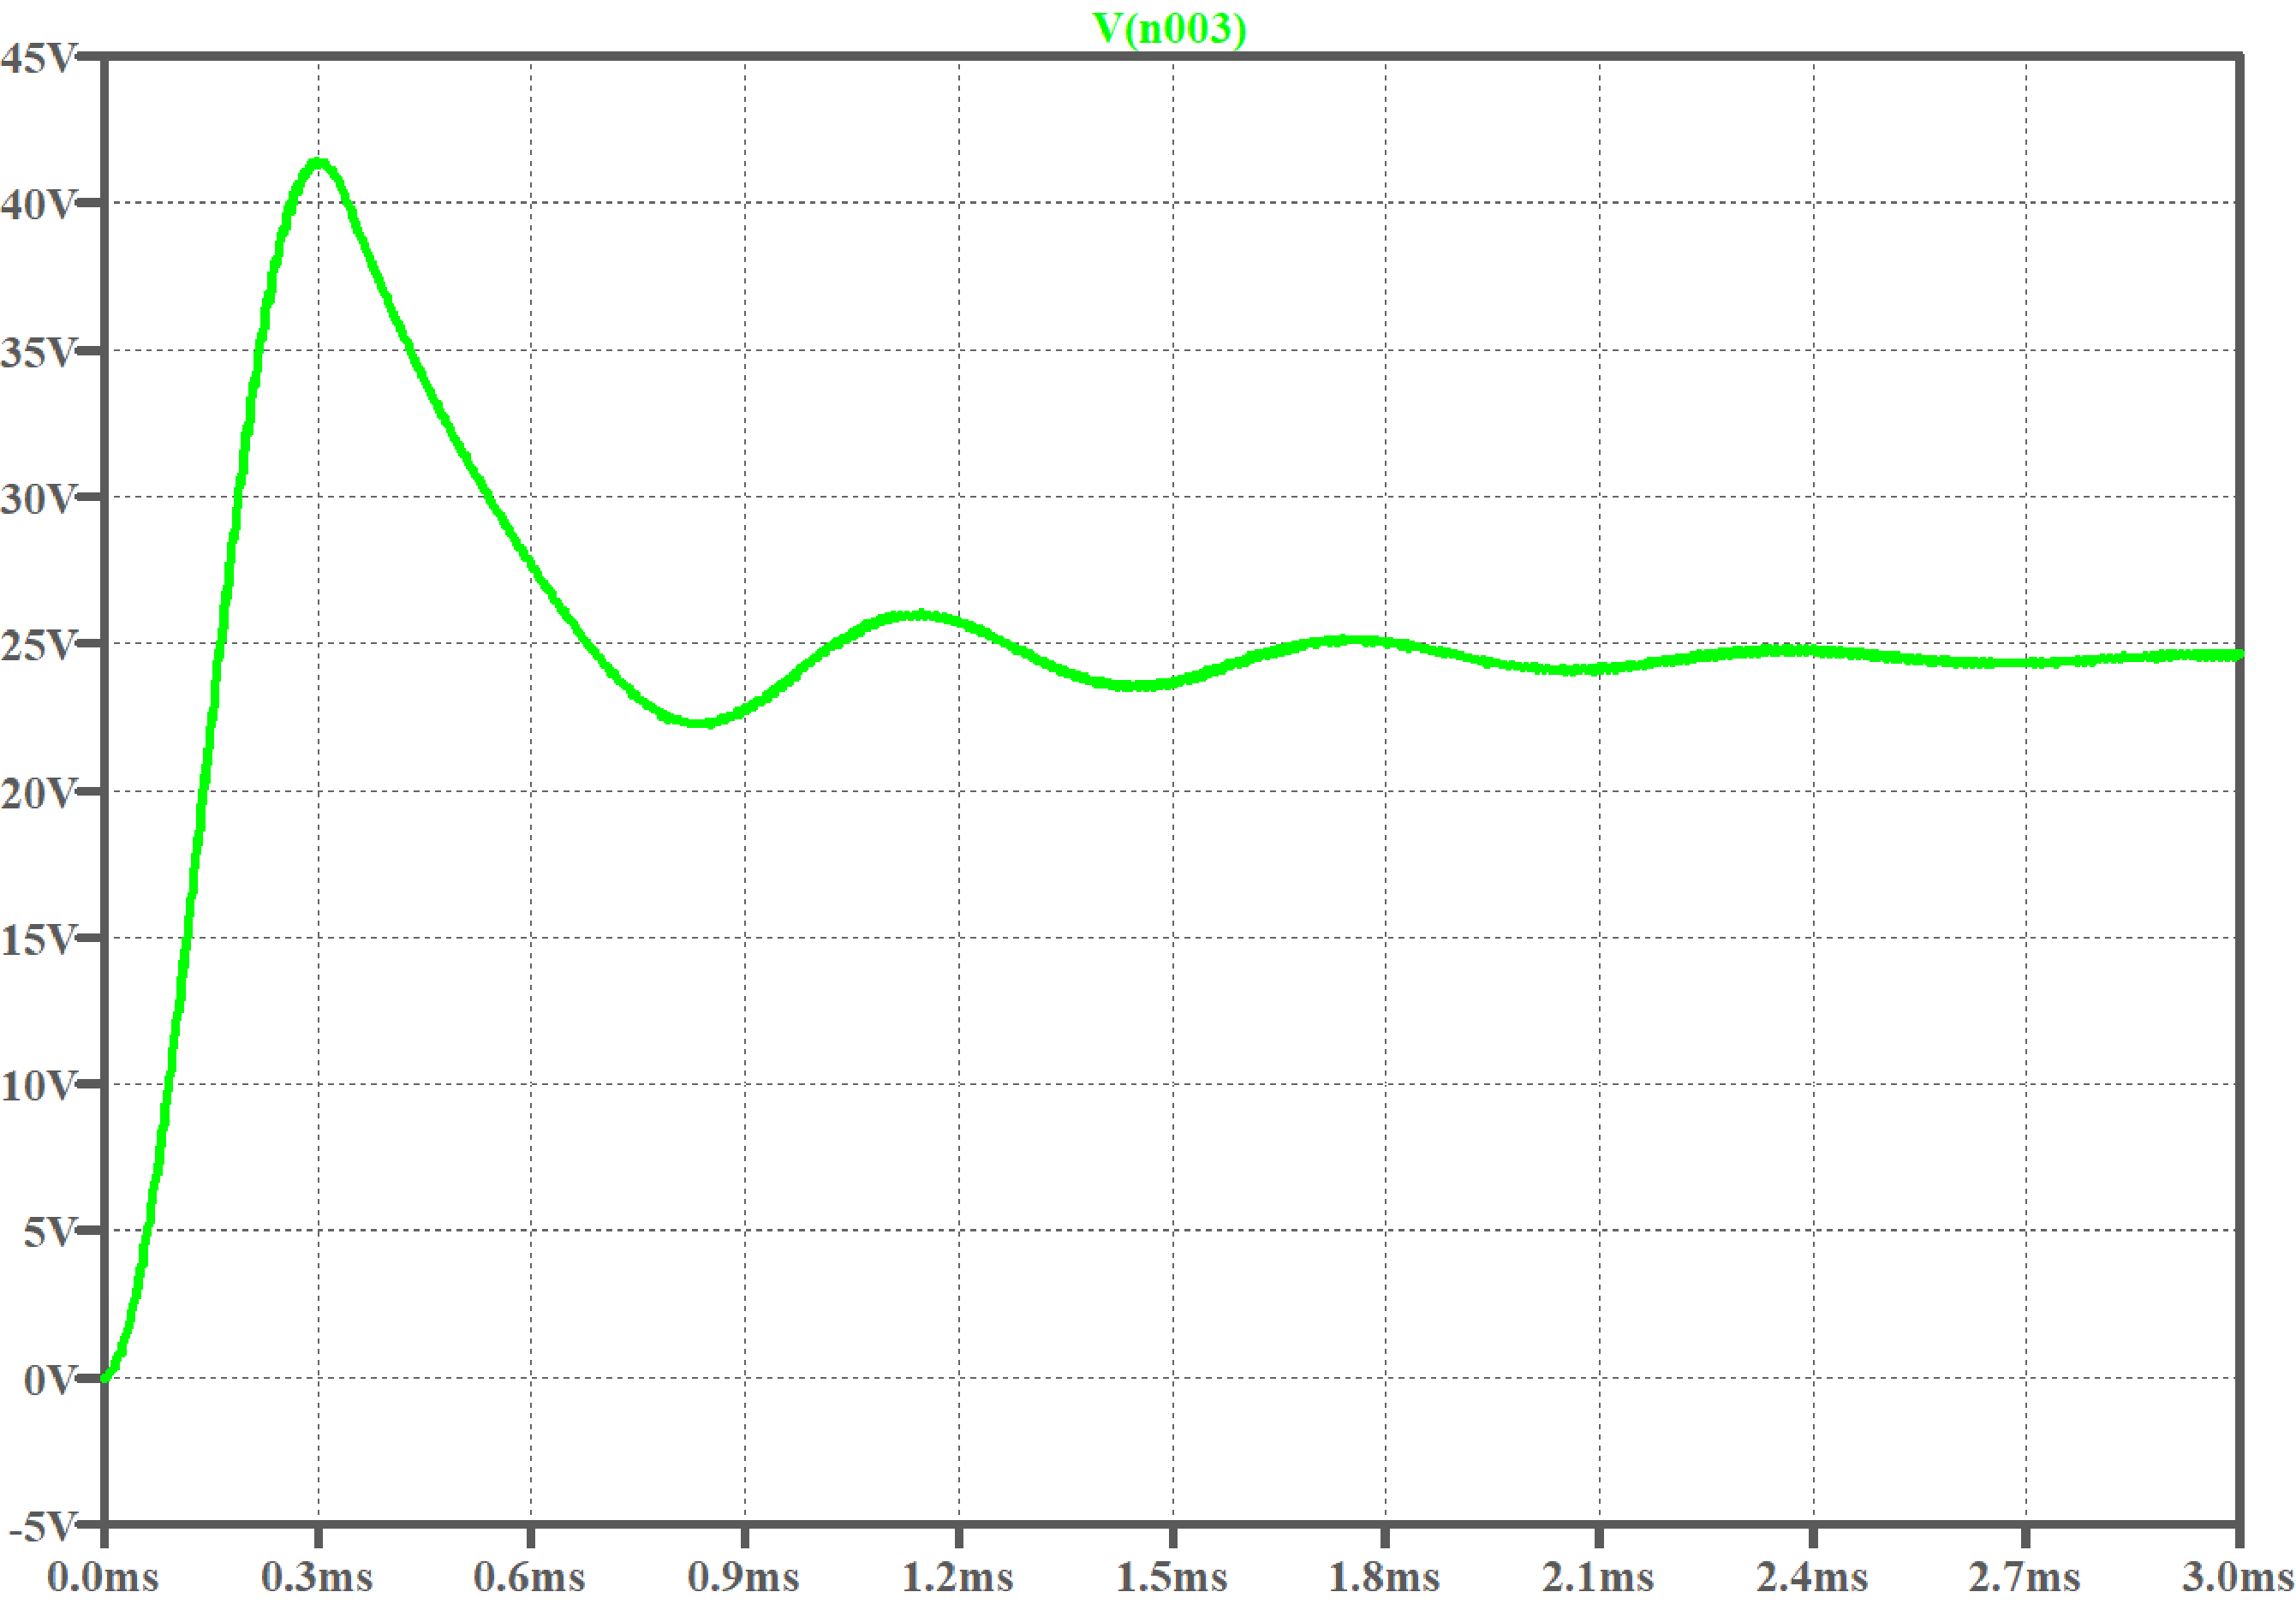
\includegraphics[width=0.55\linewidth]{Pictures/pics/LT_output_voltage.pdf}
    \caption{\textcolor{blue}{\textit{\footnotesize Flyback Converter Output Voltage Wave Form}}}
\end{figure}
\begin{figure}[h!]
    \centering
    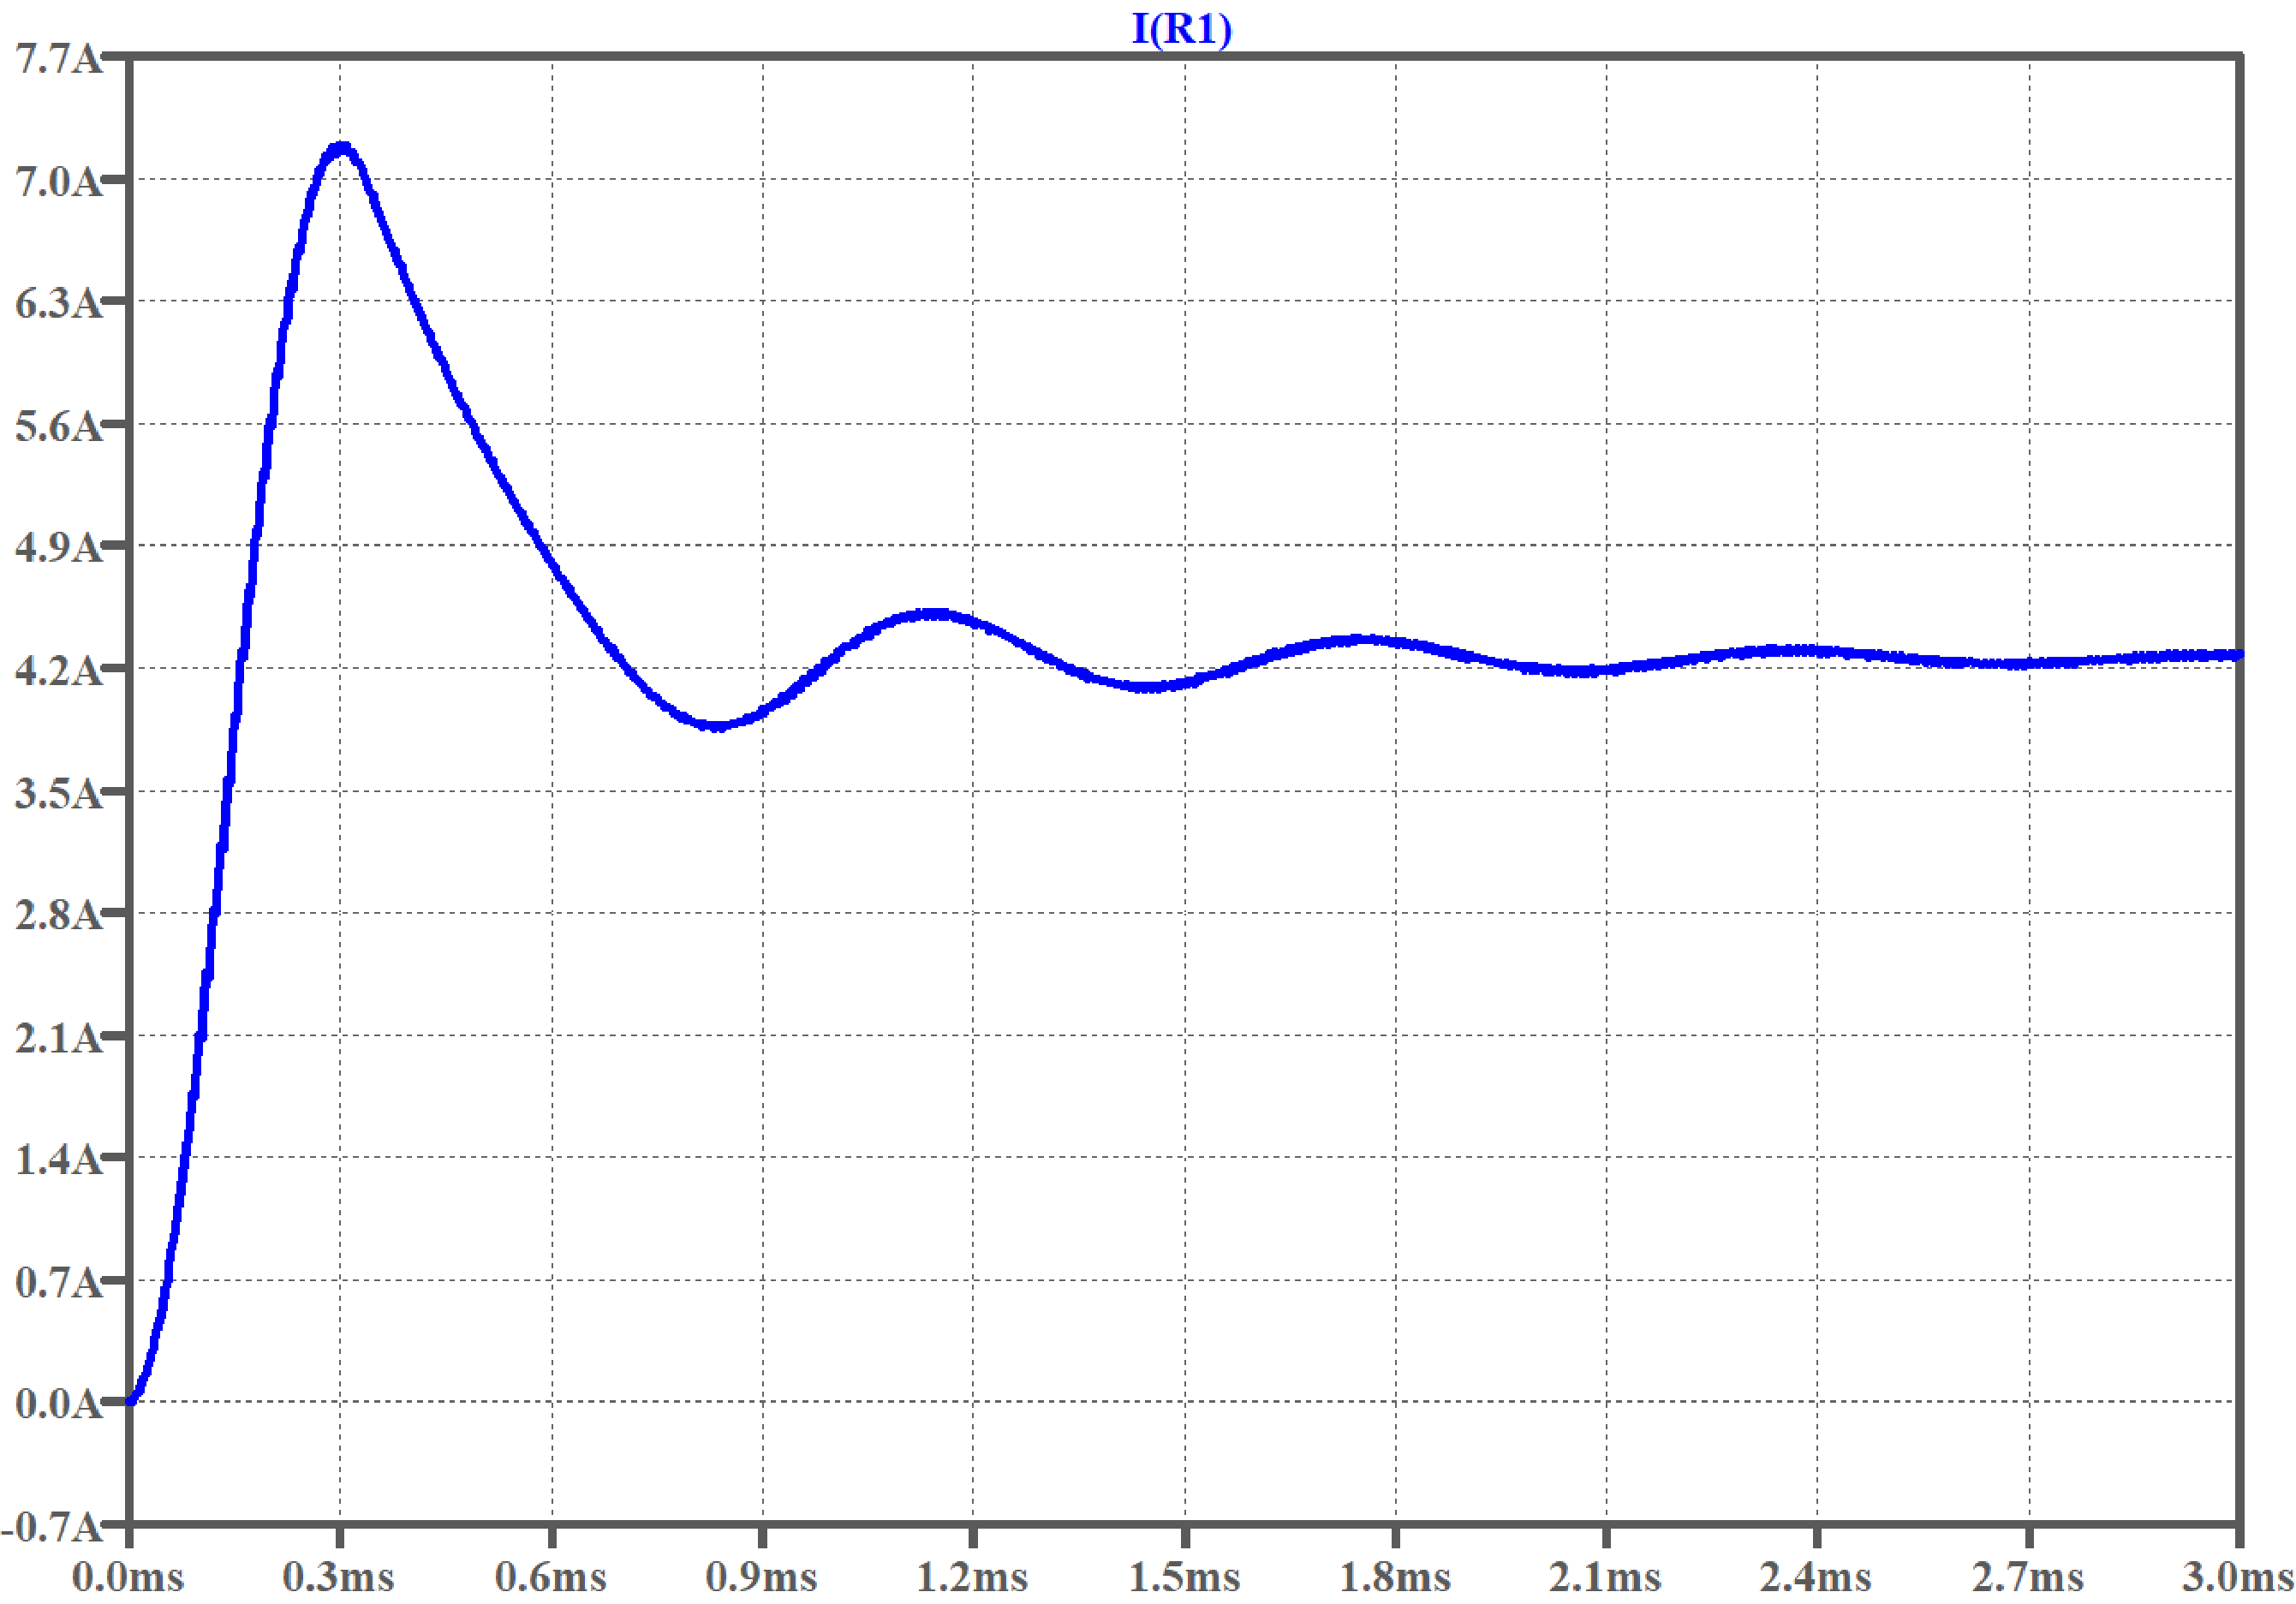
\includegraphics[width=0.55\linewidth]{Pictures/pics/LT_output_current.pdf}
    \caption{\textcolor{blue}{\textit{\footnotesize Flyback Converter Output Voltage Wave Form}}}
\end{figure}
\begin{figure}[h!]
    \centering
    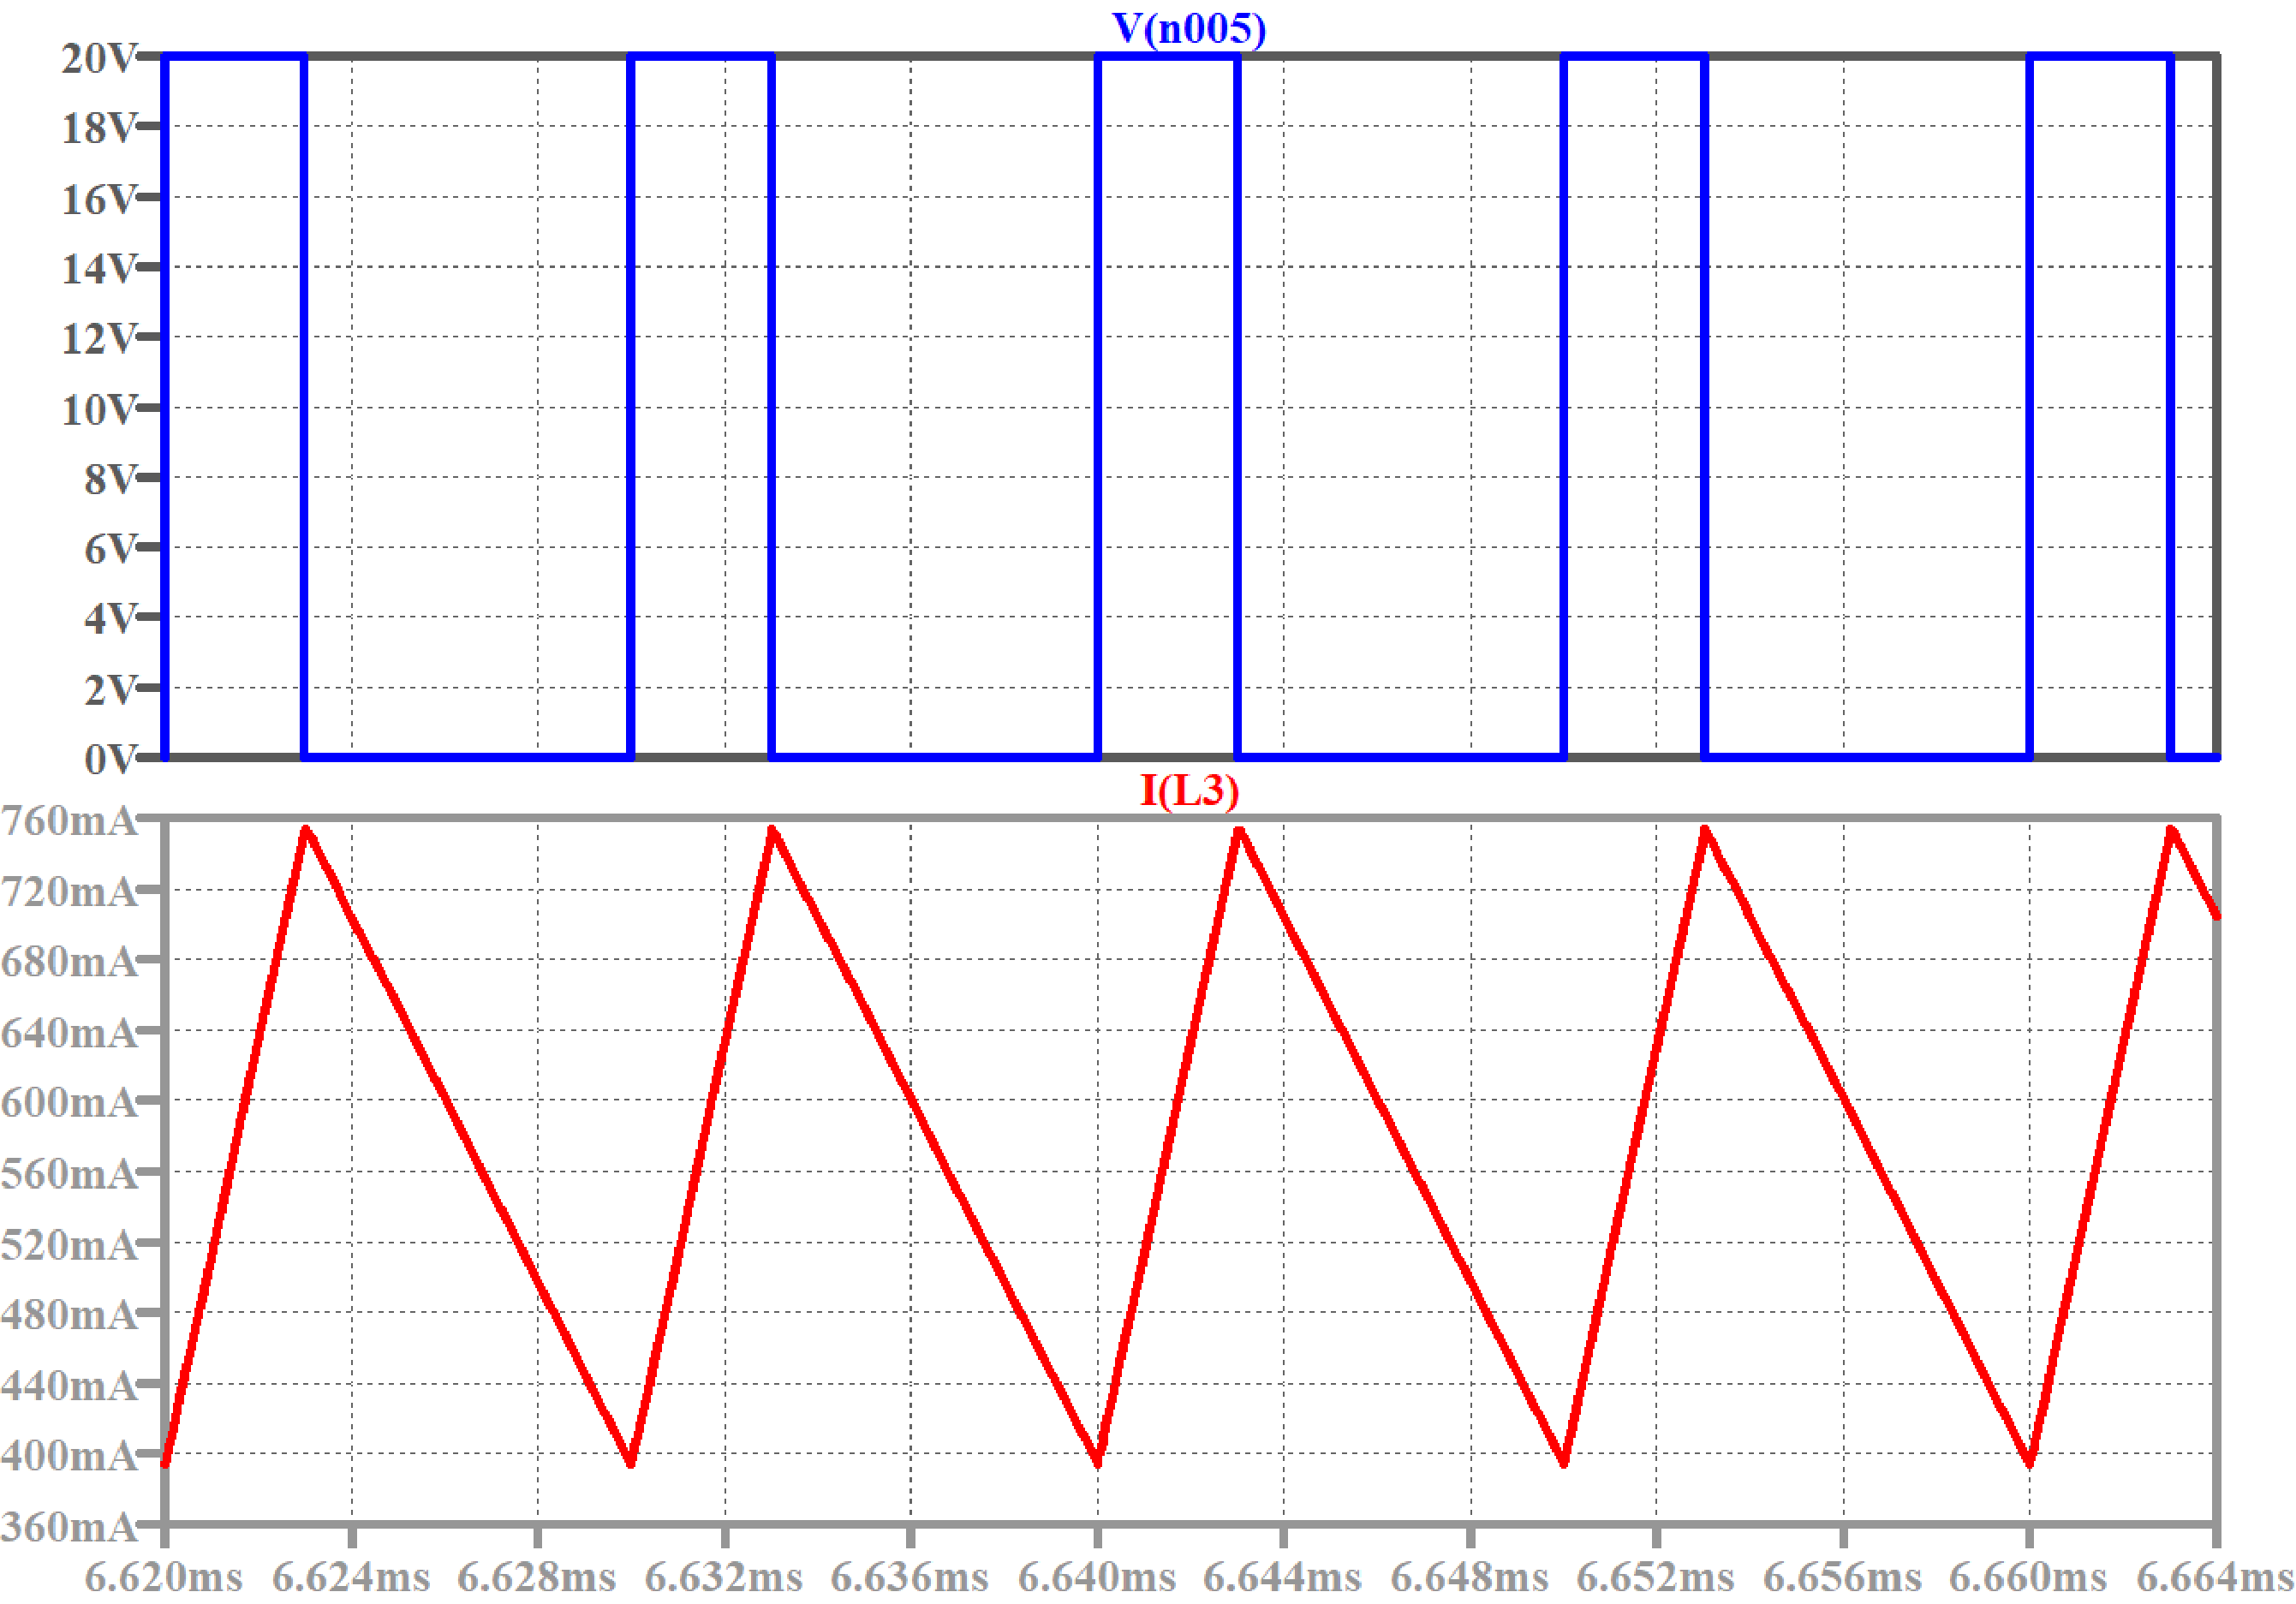
\includegraphics[width=0.7\linewidth]{Pictures/pics/L_inductance_current.pdf}
    \caption{\textcolor{blue}{\textit{\footnotesize Flyback Converter Output Voltage Wave Form}}}
\end{figure}